\documentclass[a4paper]{article}
\usepackage[utf8]{inputenc}
\usepackage{geometry}
\usepackage{amsmath}
\pdfpagewidth
\paperwidth
\pdfpageheight
\paperheight
\usepackage{booktabs}
\usepackage{graphicx}
\usepackage{subfig}
\usepackage{verbatim}
\newcommand*{\unit}[1]{\ensuremath{\mathrm{\,#1}}}
\usepackage{amsthm}
\usepackage{epsfig}
\usepackage{fancyhdr} 
\usepackage{amsmath,amssymb}
\usepackage{amscd} 
\usepackage[T1]{fontenc} 
\usepackage[utf8]{inputenc} 
\usepackage[usenames,dvipsnames]{xcolor}
\usepackage{graphicx,color,listings}
\usepackage{hologo}
\frenchspacing 
\usepackage{float}
\usepackage{geometry}
\usepackage{rotating}
\usepackage{caption}
\captionsetup{labelformat=empty, textfont=sl}
\usepackage{placeins}
\usepackage{hyperref}
\frenchspacing
\title{Esperienza Laboratorio di Fisica Medica: Spettroscopia}
\author{Simone Lossano, Lorenzo Marini, Jake Harold Pensavalle}
\begin{document}
	\maketitle
	\newpage
	\tableofcontents
	\newpage
%%%%%%%%%%%%%%%%%%%%%%%%%%%%%%%%%%%%%%
\section{Linearità, risoluzione energetica e calibrazione}
Nella prima parte di questa esperienza, abbiamo preso dimestichezza con la strumentazione, andando ad acquisire lo spettro delle sorgenti radioattive alla distanza fissata di $476 \pm 1 mm$ sulla scala millimetrata alla base del setup, mentre la superficie del rivelatore si trova a $66 \pm 1 mm$.
Prima di tutto si verifica la linearità di riposta del rivelatore, registrando un certo numero di spettri e andando a controllare che i picchi siano all'energie aspettate e che rispettino una legge lineare. 
Note le energie delle sorgenti, andiamo a calibrare la scala del multicanale trovando una relazione che fornisce CHN(E) e, tramite la relazione inversa E(CHN), troviamo la scala del multicanale calibrata in energia.
\begin{center} 
		
		\begin{tabular}{lcc}
			\hline
			\hline
			\textbf{Isotopo}	& \textbf{Energia dei Fotopicchi [KeV]} 	 \\
			\hline
			\hline
			Am241	&60 	\\
			Na22	&511,1274\\
			Cs137	&662 \\
			Co60	&1174,1323\\
			
			\hline
			\hline
		\end{tabular}
		\linebreak
		\emph{Tab.1: Energie dei fotopicchi dei vari isotopi.} 
	\end{center}
La calibrazione viene eseguita tramite una funzione di fit lineare i cui parametri sono riportati nella tabella (2):

	\begin{center} 
		
		\begin{tabular}{lcccc}
			\hline
			\hline
			\textbf{Coefficiente lineare}	& \textbf{intercetta}	& \textbf{$\chi^{2}_{redux}$} & \textbf{pvalue} \\
			\hline
			\hline
			 $0.737	\pm 0.005$	& $-16.37 \pm 0.1	$			& 0.2 &0.998	\\
			
			\hline
			\hline
		\end{tabular}
		\linebreak
		
	\end{center}
	\emph{Tab.2: risultati del fit. Il valore non ottimale del chi quadro è dovuto al fatto che si sono usati pochi punti per il fit.} 
\begin{figure}[H]%
    \centering
    \subfloat[]{{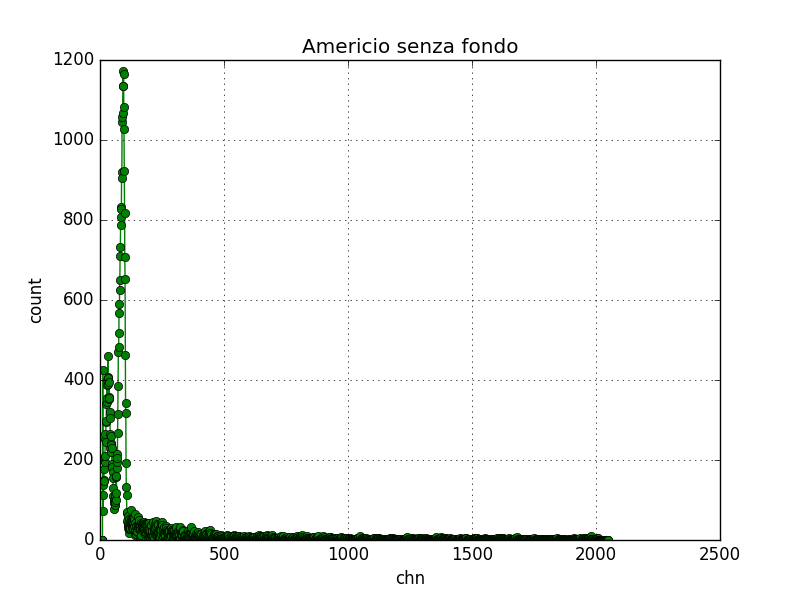
\includegraphics[width=5cm]{americio_senza_fondo} }}%
    \qquad
    \subfloat[]{{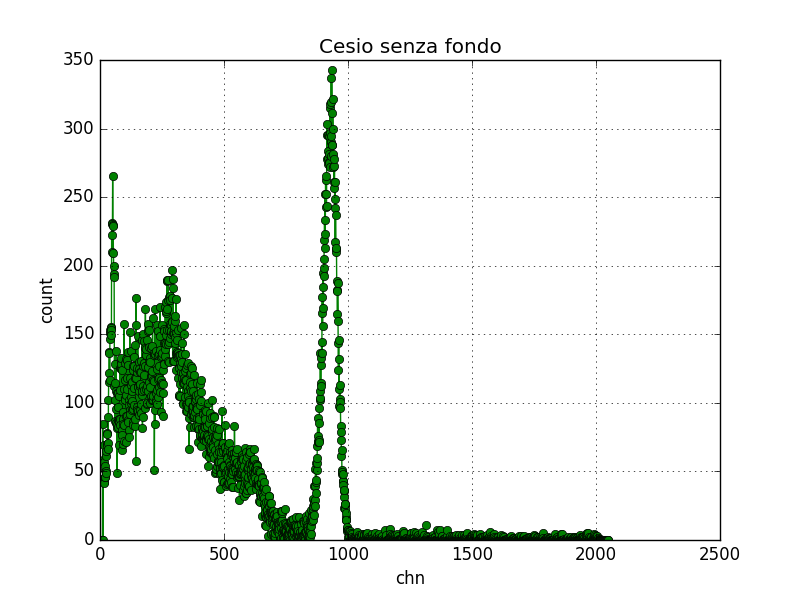
\includegraphics[width=5cm]{cesio_senza_fondo} }}%
    \qquad
    \subfloat[]{{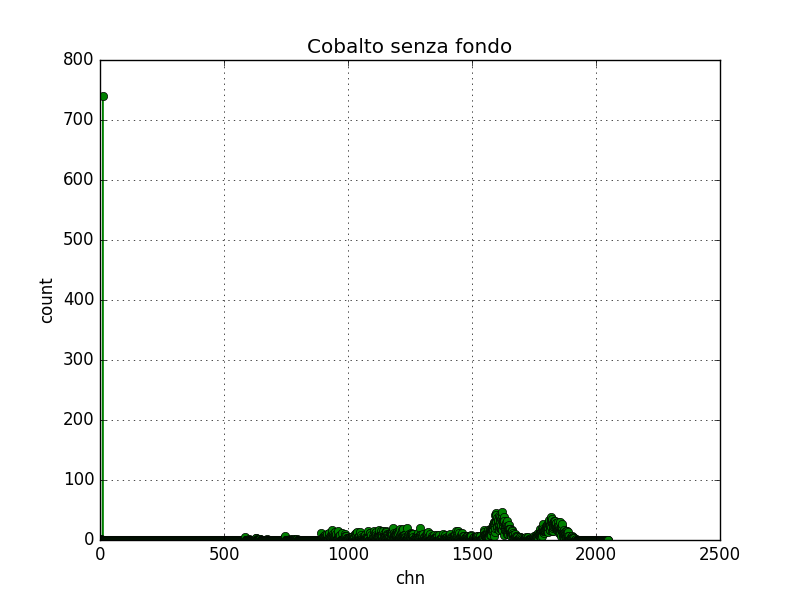
\includegraphics[width=5cm]{cobalto_senza_fondo}}}%
    \qquad
    \subfloat[]{{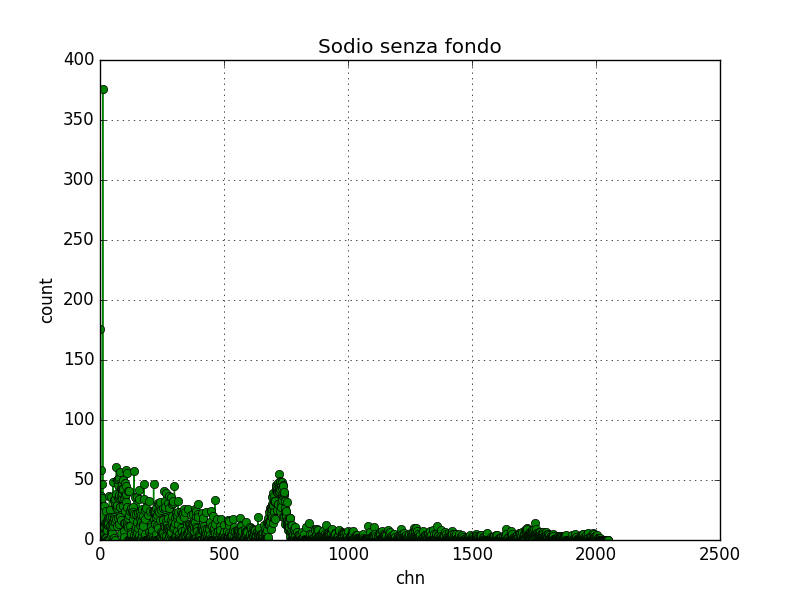
\includegraphics[width=5cm]{sodio_senza_fondo}}}%
    \qquad
    \subfloat[]{{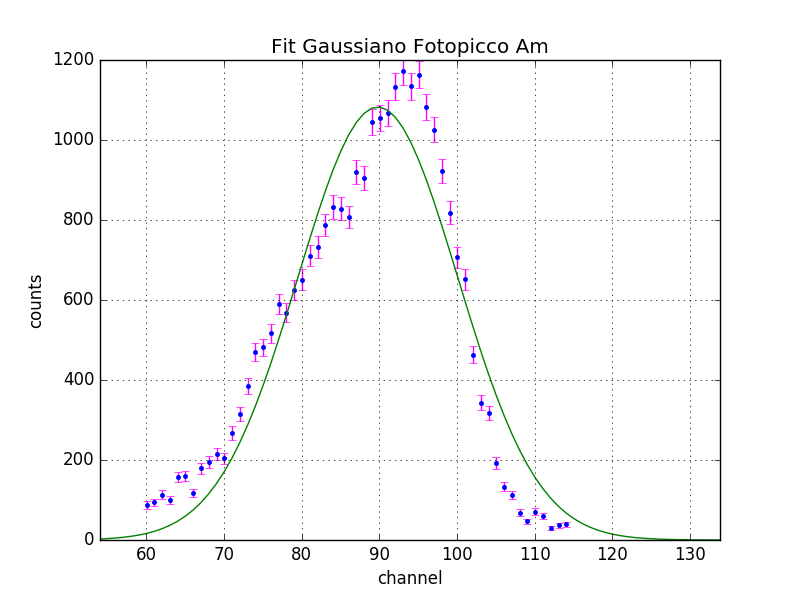
\includegraphics[width=5cm]{fit_gaussiano_Americio}}}%
    \qquad
    \subfloat[]{{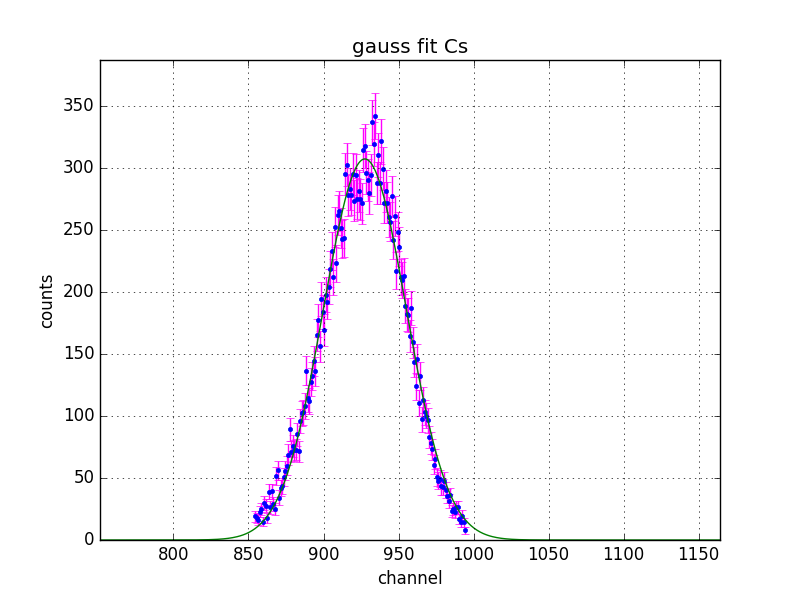
\includegraphics[width=5cm]{fit_gaussianocesio}}}%
    \qquad
    \subfloat[]{{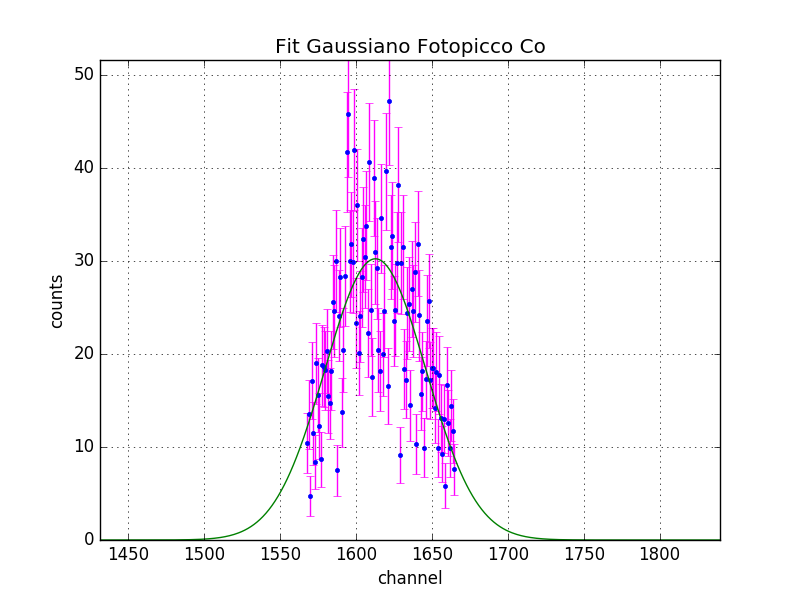
\includegraphics[width=5cm]{fit_gaussiano_cobalto1} }}%
    \qquad
    \subfloat[]{{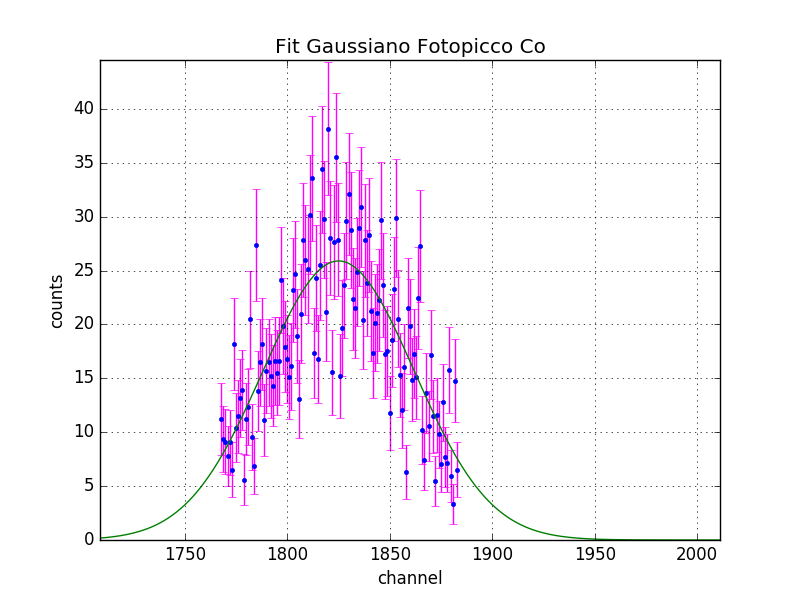
\includegraphics[width=5cm]{fit_gaussiano_cobalto_secondo_picc} }}%
    \qquad
    \subfloat[]{{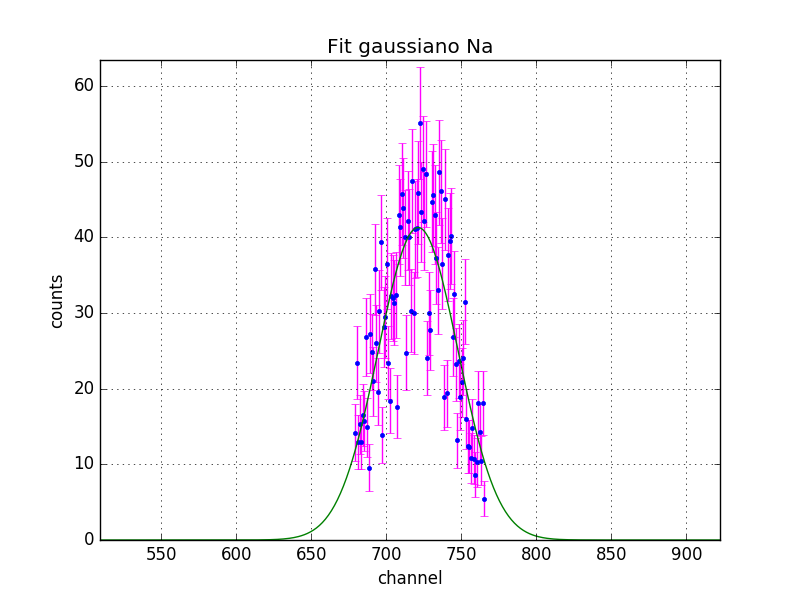
\includegraphics[width=5cm]{fit_gaussiano_Na}}}%
   \caption{Grafici degli spettri a cui è stato sottratto opportunamente il fondo e fit gaussiani dei picchi. In particolare, si riconoscono nello spettro del Cs137 l' X-Ray Photopeak e il picco di backscatter. Del Co60 si distinguono entrambi i picchi mentre per il Na22 la statistica non è sufficiente per distinguere il secondo picco con il metodo del fit gaussiano. In generale i risultati ottenuti per questi ultimi due elementi possono essere migliorati tramite acquisizioni più lunghe e sottraendo il continuum oltre al fondo acquisito.}%
    \label{fig:1}%
\end{figure}
Dai fit gaussiani si può ricavare la risoluzione energetica, usando la FWHM.
\begin{center} 
		
		\begin{tabular}{lcc}
			\hline
			\hline
			\textbf{Isotopo}	& \textbf{Risoluzione energetica [KeV]} 	 \\
			\hline
			\hline
			Am241	&26.496	\\
			Na22	&61.450\\
			Cs137	&70.730 \\
			Co60	&78.069,85.875\\
			
			\hline
			\hline
		\end{tabular}
		\linebreak
		\emph{Tab.3:Risoluzione energetica dei vari isotopi.} 
	\end{center}
\begin{figure}[!h]
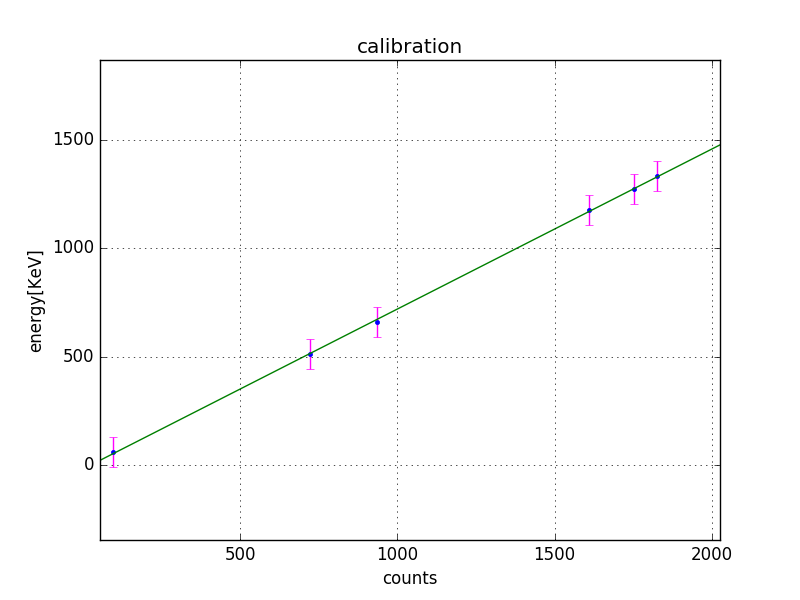
\includegraphics[width=1\textwidth]{calibrazione}
        \caption{Calibrazione del rivelatore. Il punto corrispondente al secondo picco del sodio è stato stimato visivamente nello spettro}
        \label{fig:2}
\end{figure}


\pagebreak


\section{Verifica di 1/$r^2$}
In questa sezione si verifica l'andamento del rate dei conteggi in funzione della distanza della sorgente dal rivelatore. Per il calcolo dei conteggi ed il fit è stata considerata l'area sotto il fotopicco in quanto corrispondente al numero totale dei conteggi sotto al picco. Si sono eliminati gli outlier corrispondenti alle distanze più piccole tra sorgente e rivelatore, poichè, come aspettato, stando troppo vicino a quest'ultimo, vi sono fenomeni di pile-up che rendono invalide tali acquisizioni. Come modello si è utilizzato \begin{equation}
A_{fotopicco}=\frac{C}{r^{2}}+B
\end{equation}
Con A e B parametri stimati dal fit.
\begin{figure}[H]
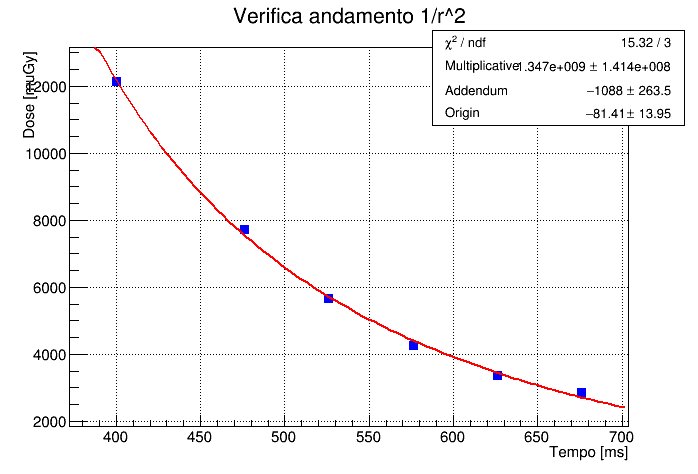
\includegraphics[width=1\textwidth]{inverserootlawwithpars}
        \caption{Andamento area sotto il fotopicco in funzione della distanza.}
        \label{fig:2}
\end{figure}

\section{Calcolo di $\mu$/$\rho$ di Cu e di Al}
Si voglioni studiare i $\mu$ di attenuazione di rame e alluminio. La misura viene fatta con una sorgente di Cs137 (in quanto presenta un unico fotopicco ed ha un'attività sufficiente per ottenere un buon numero di acquisizioni), frapponendo vari spessori dei materiali. La misura viene fatta per il Cu e successivamente con Al, la sorgente è stata posta ad una distanza di $400  \pm 1mm$. Per la misura del $\mu$ del Cu, i dischi sono stati posti su un supporto collimatore (il più possibile vicino alla sorgente) e la prima acquisizione è stata fatta con la sola presenza del supporto senza spessori.  La funzione di fit utilizzata è:
\begin{equation}
A_{fotopicco}=A_{0}e^{-\mu x} + B
\end{equation}
Con $A_{0}$ e B parametri liberi.

\begin{center} 
		
		\begin{tabular}{lccccc}
			\hline
			\hline
			\textbf{Materiale}&\textbf{$\mu$ }	& \textbf{costante additiva}	& \textbf{$\chi^{2}_{redux}$} & \textbf{pvalue} \\
			\hline
			\hline
			 Cu&$0.575	\pm 0.009$	& $14068.144 \pm 78.833	$			& 1.8 &0.113	\\
			Al&$0.194 \pm 0.06$ &$10553 \pm 148.143$ & 8.213 & 0.000 \\
			\hline
			\hline
		\end{tabular}
		\linebreak
		
	\end{center}
	\emph{Tab.4: risultati del fit esponenziale. Il valore non ottimale del chi quadro è dovuto al fatto che si sono usati pochi punti per il fit, limitati dal numero di spessori utilizzati.} 
\begin{figure}[H]%
    \centering
    \subfloat[]{{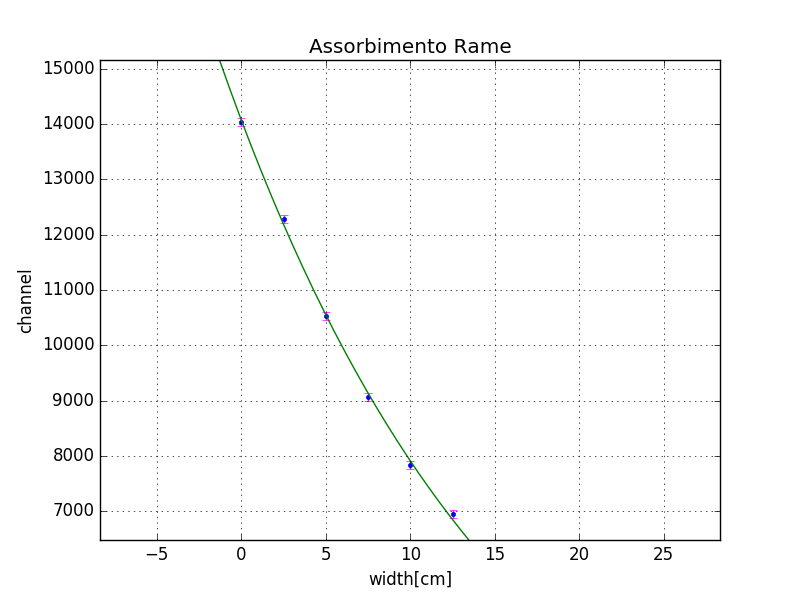
\includegraphics[width=6cm]{assorbimento_rame} }}%
    \qquad
    \subfloat[]{{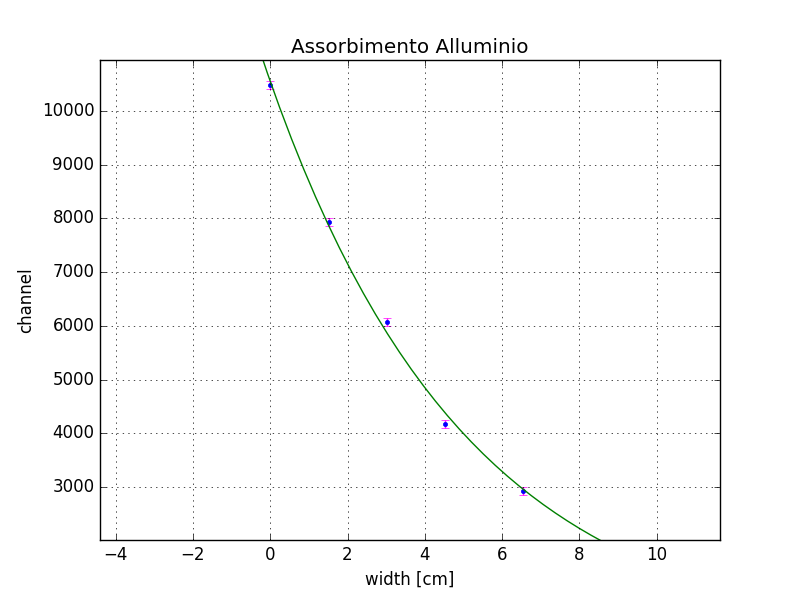
\includegraphics[width=6cm]{assorbimento_alluminio} }}%
    
   \caption{Grafici assorbimento del rame e dell'alluminio.}%
    \label{fig:1}%
\end{figure}
\subsection{Confronto $\frac{\mu}{\rho}$ tra dati sperimentali e tabulati}
Conoscendo la densità del materiale si può stimare il rapporto $\frac{\mu}{\rho}$:
\begin{center} 
		
		\begin{tabular}{lccc}
			\hline
			\hline
			\textbf{Materiale}&\textbf{$\frac{\mu}{\rho}_{exp} [\frac{cm^{2}}{gr}] $}	& \textbf{$\frac{\mu}{\rho}_{theo}[\frac{cm^{2}}{gr}] $}	 \\
			\hline
			\hline
			 Cu&$0.065 \pm 0.001	$	& $0.066$			\\
			Al&$0.072 \pm 0.003$ &$0.068$ \\
			\hline
			\hline
		\end{tabular}
		\linebreak
		
	\end{center}
	\emph{Tab.5: Confronto tra valori sperimentali e valori attesi. Possiamo notare un buon accordo tra i valori.} 

\section{Calcolo dell'efficienza intrinseca di picco in funzione dell'energia}
Utilizzando una attività al tempo zero nominale di 74 kBq e usando come tempo di riferimento il giorno 18/02/05 (t= 14.72 yr), si possono calcolare le attività e si possono calcolare le efficienze utilizzando:
\begin{equation}
\epsilon_{int}=\epsilon_{abs}4 \frac{\pi}{\omega}
\end{equation}
Dove $\omega$ è l'accettanza geometrica stimata dalla geometria del sistema, ed $\epsilon_{abs}$=$\frac{# eventi rilevati }{# eventi totali}$ dove il numero di eventi totali si stima sapendo l'attività e i tempi di misura.
\begin{center} 
		
		\begin{tabular}{lcc}
			\hline
			\hline
			\textbf{Isotopo}	& \textbf{Attività [KBq]} 	 \\
			\hline
			\hline
			Am241	&71.478 	\\
			Na22	&0.23\\
			Cs137	&45.39\\
			Co60	&4.30\\
			
			\hline
			\hline
		\end{tabular}
		\linebreak
		\emph{Tab.6: Attività dei vari isotopi.} 
	\end{center}
\begin{figure}[H]
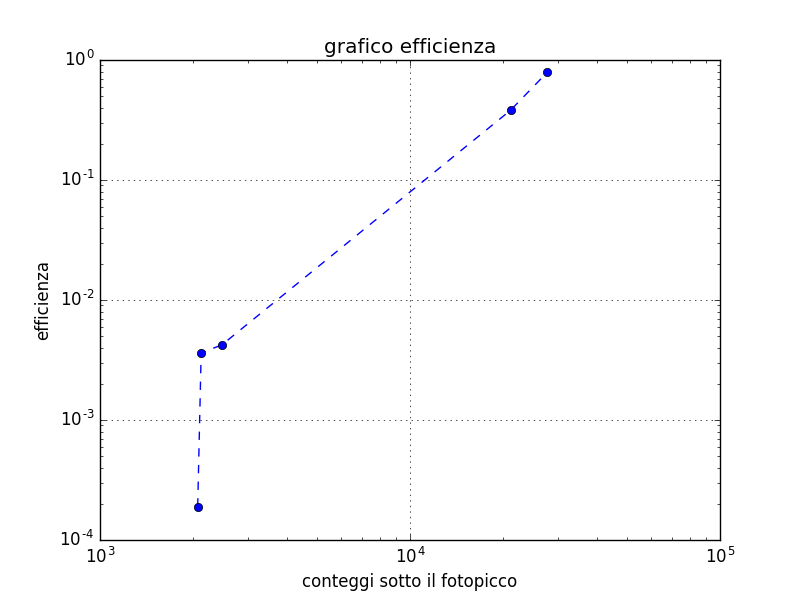
\includegraphics[width=1\textwidth]{efficiency}
        \caption{Efficienza in funzione dell'energia. Le scarse efficienze per il Co e Na sono dovute alla statistica non ottimale per quei punti. Per un migliore confronto con il plot di riferimento sul manuale del rivelatore, si rimanda ad un'acquisizione dati sufficiente per tali sorgenti.}
        \label{fig:2}
\end{figure}
\section{Referenze}
Il repositorio su GitHub in cui vi sono immagini, programmi Python e Root è
https://github.com/Jake145/Gruppo-3-Lab-Fisica-Medica.git

\end{document}